\PassOptionsToPackage{unicode}{hyperref}
\documentclass[aspectratio=1610, professionalfonts, 9pt]{beamer}

\usefonttheme[onlymath]{serif}
\usetheme[showtotalframes]{tudo}

\ifluatex
  \usepackage{polyglossia}
  \setmainlanguage{german}
\else
  \ifxetex
    \usepackage{polyglossia}
    \setmainlanguage{german}
  \else
    \usepackage[german]{babel}
  \fi
\fi

\newcommand*\xRightarrow[2][]{\ext@arrow 0359\Rightarrowfill@{#1}{#2}}

% Mathematik
\usepackage{amsmath}
\usepackage{amssymb}
\usepackage{mathtools}
\usepackage{cancel}

\usepackage{hyperref}
\usepackage{bookmark}
\usepackage{siunitx}
\usepackage{overpic}
%%%%%%%%%%%%%%%%%%%%%%%%%%%%%%%%%%%%%%%%%%%%%%%%%%%%%%%%%%%%%%%%%%%%%%%%%%%%%%%%
%%%%%-------------Hier Titel/Autor/Grafik/Lehrstuhl eintragen--------------%%%%%
%%%%%%%%%%%%%%%%%%%%%%%%%%%%%%%%%%%%%%%%%%%%%%%%%%%%%%%%%%%%%%%%%%%%%%%%%%%%%%%%

%Titel:
\title{Stromnetz und Strombörse}
%Autor
\author[D.~Hering]{Dag-Björn Hering}
%Lehrstuhl/Fakultät
%\institute[Experimental Physics 5]{Names des Lehrstuhls \\  Name der Fakultät}
%Titelgrafik
\titlegraphic{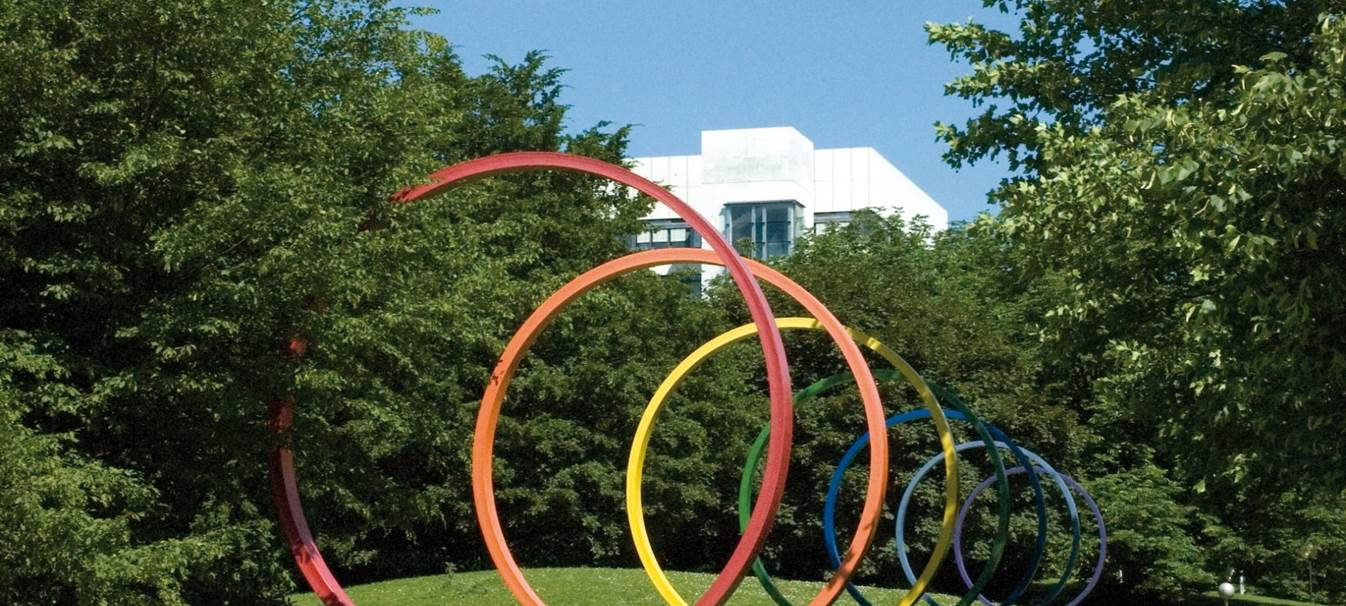
\includegraphics[width=0.7\textwidth]{images/tudo-title-2.jpg}}


\begin{document}
\maketitle

\begin{frame}{Gliederung}
\begin{itemize}
  \item Stromnetz
  \begin{itemize}
  \item Vorderungen an das Stromnetz
  \item Frequenz im Netz
  \item Reguationsmechanismen der Frequenz
  \item Spannungsebenen
  \item Verteilung
  \item Netzbetreiber
  \item Anspruch an das Stromnetz durch die Energiewende
  \end{itemize}
\end{itemize}
\end{frame}

\begin{frame}
\begin{itemize}
 \item Strombörse
\begin{itemize}
  \item Enwicklung der Strombörse
  \item Angebote der Strombörse
  \item Spot Markt(und seine Folgen auf das Netz)
  \item Strompreis aus der Merit Order
  \item EEG-Umlage
  \item Strompreisentwicklung
\end{itemize}
\end{itemize}
\end{frame}




\begin{frame}{Stromnetz-Historisch}
\begin{itemize}
  \item Beginn der Elektrifizierung 1880 mit der Industrialisierung
  \item zunächst nur Inselnetze mit Gleichstrom zur Beleuchtung
  \item Wechselstrom setzte sich gegen Gleichstrom wegen Vorteilen wie
  \begin{itemize}
    \item[-] damals Transformator einzige Möglichkeit Hochspannung zu erzeugen
    \item[$\rightarrow$] einfaches Umspannen von Hochspannung zu Verbraucherspannung möglich
    somit weniger Verluste bei langen Leitungen und "sichere" Niederspannung bei Verbraucher
    \item[-] große Verbundnetze möglich, die aber alle synchron mit gleicher Frequenz betrieben werden.
  \end{itemize}
  \item heutige Verbundnetze werden mit $\SI{50}{\hertz}$ bzw. $\SI{60}{\hertz}$ Drehstrom(Dreiphasiger Wechselstrom) betrieben
  \item Nur vereinzelt Gleichstrom (z. B. bei Verkehr und HGÜ) jedoch wieder steigend
\end{itemize}
\end{frame}
%

\begin{frame}{Dreiphasiger Wechselstrom}
  \begin{columns}
    \begin{column}{0.5\textwidth}
\begin{itemize}
  \item Drei Wechselströme die um $\SI{120}{\degree}$ zueinander verschoben sind
  \item einfache Erzeugung durch Drehstromgenerator
  \item Steckdose im Zuhaus benutzten jeweils nur eine der drei Wechselströme
  \item Bzw. Öfen und Motoren nutzen alle drei Phasen( konstant Leistung )
  \item Materialaufwand für Leitung geringer als bei einphasiger Wechselstrom bei gleicher Leistung,
   da Phasen in seperaten Kabeln geführt werden
  \item Besitzt zwei abgreifbare Spannungen  Nennspannung(Phase-Phase) und Phasenspannung(Phase-Null)
\end{itemize}
\end{column}
\begin{column}{0.5\textwidth}
  \begin{figure}
\includegraphics[width=0.9\textwidth]{images/Drehstromgenerator.jpg}
%www.c-turbines.ch
\end{figure}
\end{column}
\end{columns}
\end{frame}

{
\setbeamertemplate{footline}{}
\begin{frame}{Europäisches Verbundsystem}
\begin{columns}
\begin{column}{0.5\textwidth}
\begin{itemize}
\item besteht aus mehrere voneinander getrennte Verbundsysteme
\item Verbundsystem:
Zusammenschluss von Höchst und Hochspannungsnetzen der Länder zur z. B. UCT  (Union for the Co-ordination of the Transmission of Electricity)
%\item Verbundnetze werden mit Drehstrom betrieben (Drehstrom $\stackrel{^}{=}$ 3-phasigen Wechselstrom)
\item Verband Europäischer Übertragungsnetzbetreiber
European Network of Transmission System (ENTSO-E) übernimmt Koordination
der Verbundsysteme
\end{itemize}
\end{column}
\begin{column}{0.5\textwidth}
    \begin{figure}
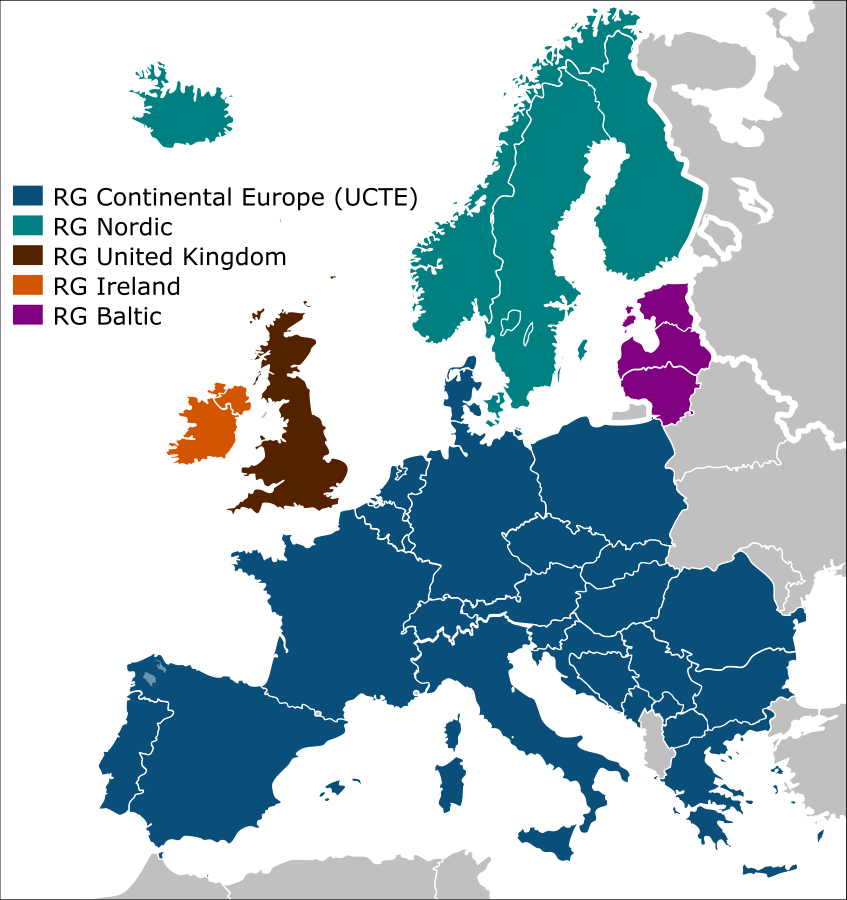
\includegraphics[width=0.9\textwidth]{images/Euronetz.png}
\end{figure}
\end{column}
\end{columns}
% Quelle: https://commons.wikimedia.org/w/index.php?curid=1387849
\end{frame}
}


  \begin{frame}

  \begin{block}{Hochspannungs-Gleichstrom-Übertragung (HGÜ)}
    \begin{itemize}
      \item dient zur Energieübertragung zwischen zwei weit entfernten Punkten
      \item ab $\SI{750}{\kilo\meter}$ effizienter als Leitungen mit Wechselstrom
  \item[] \textbf{\textcolor{tugreen}{Ursache:}} HGÜ: ohmscher Widerstand
  \item[] \textbf{\textcolor{tulight}{Ursache:}} Wechselstrom: ohmscher Widerstand, Skin-Effekt, kapazitiver Widerstand und Blindwiderstand
%Quelle:https://www.weltderphysik.de/gebiete/technik/energie/speichern-und-transportieren/strom/hochspannung/
% \begin{tabular}{c c}
%  AC    &          DC \\
% \hline
% \multicolumn{2}{c}{OhmscherWiderstand}\\
% Skin-Effekt &  - \\
% BlindWiderstand& -\\
%  \end{tabular}
% \begin{itemize}
      \item verbindet die getrennten und asynchronen Verbundsysteme Europas und bspw. Offshore-Windparks mit dem Festland
      \end{itemize}
\end{block}
\end{frame}

{
\setbeamertemplate{footline}{}
\begin{frame}
\begin{columns}
\begin{column}{0.4\textwidth}
\begin{figure}
     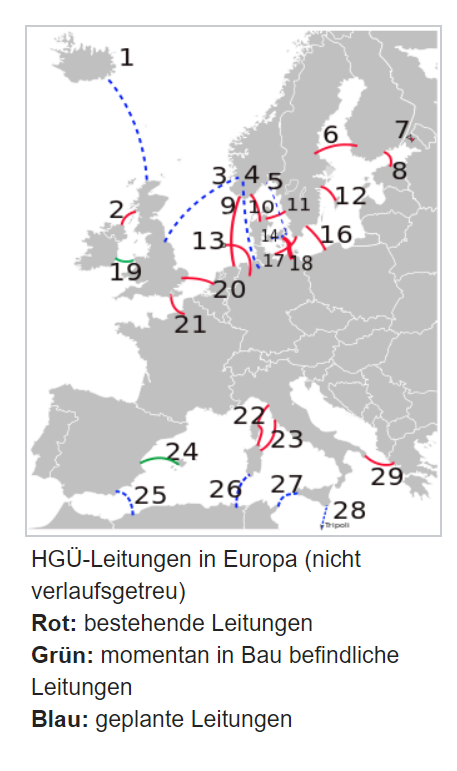
\includegraphics[width=0.9\textwidth]{images/HGUeuropa.png}
 \end{figure}
\end{column}
\begin{column}{0.6\textwidth}
  \begin{figure}
      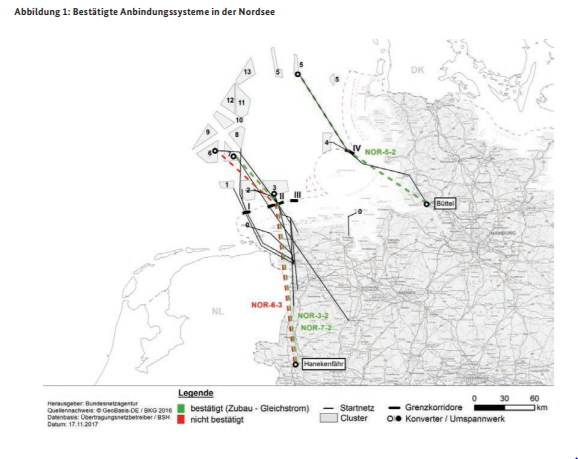
\includegraphics[width=1\textwidth]{images/HGU.PNG}
  \end{figure}
\end{column}
\end{columns}
\end{frame}
}


{
\setbeamertemplate{footline}{}
\begin{frame}
  \begin{columns}
\begin{column}{0.5\textwidth}
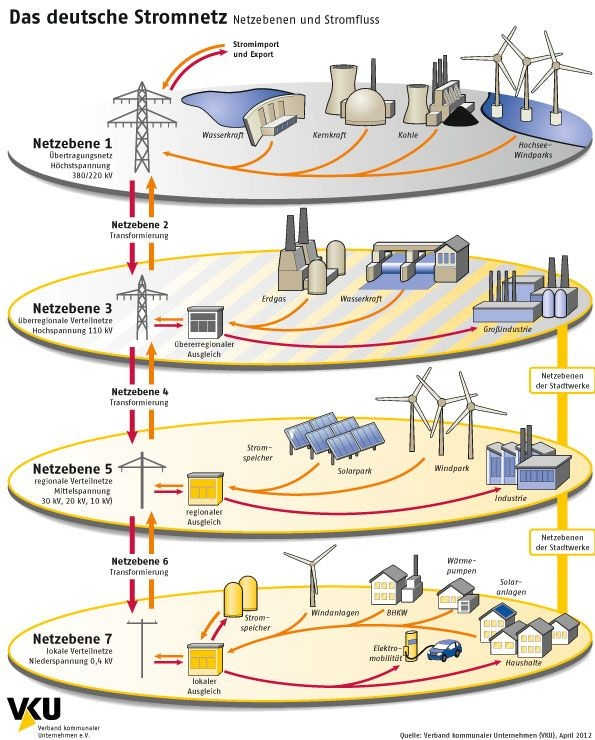
\includegraphics[width=1\textwidth]{images/netzebenen.jpg}
%Quelle: http://www.bpb.de/politik/wirtschaft/energiepolitik/148524/ausbau-des-stromnetzes
\end{column}
\begin{column}{0.5\textwidth}
  %\frametitle{Netzebenen}
  \begin{itemize}
    \item besteht aus \num{7} Netzebenen
    \item \num{4} Spannungsebenen
    \begin{itemize}
      \item[-] Höchstspannung $\num{220}$-$\SI{380}{\kilo\volt}$
      \item[-] Hochspannung  $\num{60}$-$\SI{110}{\kilo\volt}$
      \item[-] Mittelspannung  $\num{6}$-$\SI{50}{\kilo\volt}$
      \item[-] Niederspannung $\num{230}$/$\SI{400}{\volt}$
    \end{itemize}
    \item \num{3} Transformationsebenen jeweils zwischen den Spannungsebenen
  \end{itemize}
\end{column}
\end{columns}
\end{frame}
}

{
\setbeamertemplate{footline}{}
\begin{frame}
  \begin{figure}
    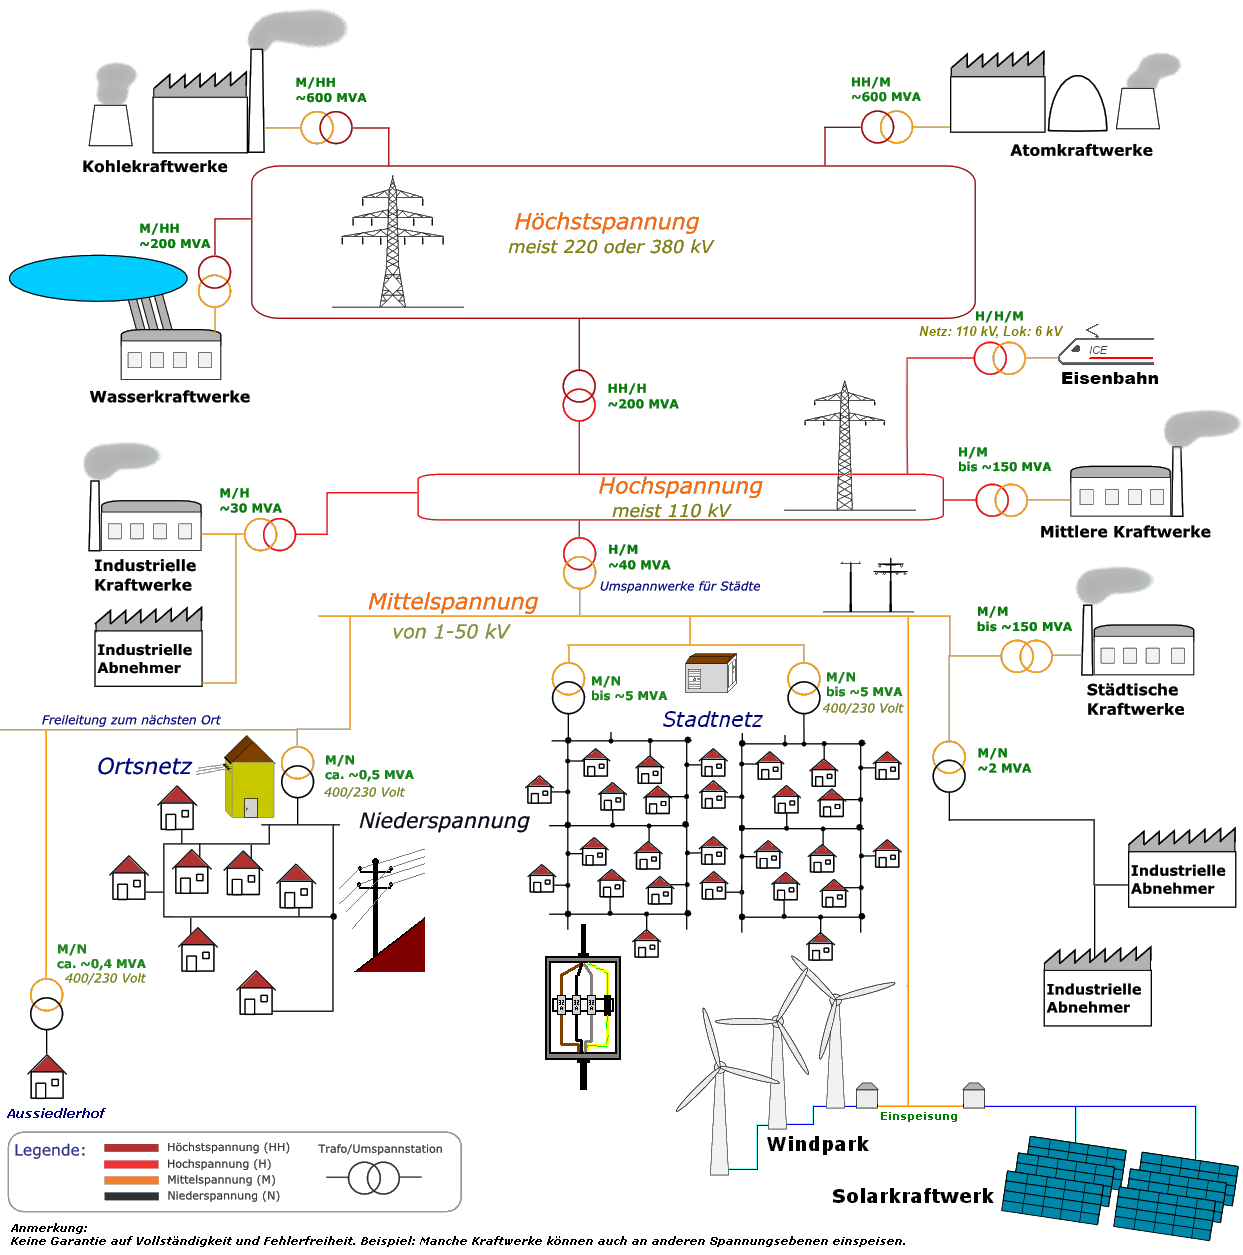
\includegraphics[width=0.6\textwidth]{images/Stromversorgung.png}
  \end{figure}
  %:Quelle:
\end{frame}
}

\begin{frame}
  \begin{itemize}
    \item Leistungsflüsse in den Netzen werden durch Änderung
      von Blind- und Wirkleistung sowie durch Phasenverschiebungen
      zur Netzstablilisierung angepasst
      (FACTS Flexible AC Transmission Systems)
    \item Höchstpannung für möglichst verlustfreie Leitung
          \begin{align*}
P_{\text{Verlust}}&= U_\text{R}\cdot I = R \cdot I^2 = \rho\cdot\frac{l}{A} \cdot I^2  \\
P_\text{ges}&=U\cdot I \Leftrightarrow I=\frac{P_\text{ges}}{U}\\
P_{\text{Verlust}}&=\rho\cdot\frac{l}{A} \cdot \frac{P_\text{ges}^2}{U^2}
          \end{align*}
  \end{itemize}
\end{frame}


\begin{frame}
  \begin{columns}
  \begin{column}{0.5\textwidth}
  \begin{itemize}
    \item Hoch-/Mittel-/Niederspannungs Ebenen
     werden regional und lokal von Verteilernetzbetreibern verwaltet
    \item die Höchstspannung Ebene teilen sich in
    Deutschland die Übertragungsnetzbetreiber
    \begin{itemize}
      \item[-] Tennet
      \item[-] 50-Hertz
      \item[-] Amprion
      \item[-] Transnet
  \end{itemize}
\end{itemize}
\end{column}
\begin{column}{0.5\textwidth}
\begin{figure}
    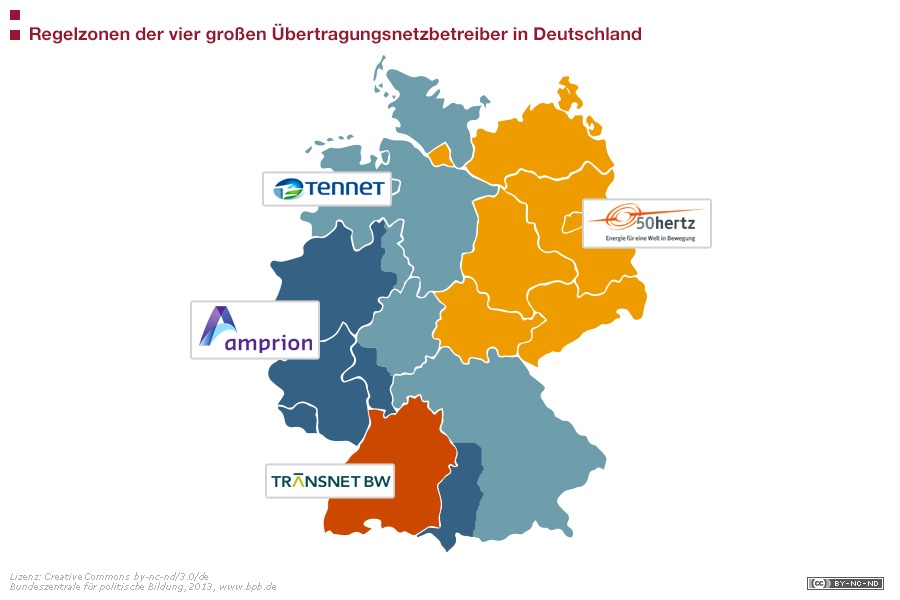
\includegraphics[width=1.1\textwidth]{images/UNB.jpg}
%Quelle:http://www.bpb.de/politik/wirtschaft/energiepolitik/148524/ausbau-des-stromnetzes
\end{figure}
\end{column}
\end{columns}
\end{frame}

\begin{frame}{Netzfrequenz}
\begin{itemize}% [<+->]
\item Richtfrequenz von $\SI{50}{\hertz}$ im europäischen Verbundnetz
\item hängt von Rotationsgeschwindigkeit der synchronisierten Generatoren
ab
% Um dieses umgangssprachlicher zu erklären, wird
% gerne der Alltagsvergleich mit einem Fahrrad herangezogen:
% Auf einer gleichmässigen Fläche kann relativ einfach eine
% konstante Trittgeschwindigkeit gehalten werden.
% An einer Steigung (zu vergleichen mit steigender Last im Stromnetz)
% muss mehr Kraft aufgewendet werden, um die Trittfrequenz
% beizubehalten oder sie kann sogar (kurzeitig) sinken,
% bis man sich auf die Steigung eingestellt hat.
% Anders herum steigt die (Tritt-)Frequenz an einem Gefälle
% kurz an, bis man sie (zum Beispiel durch Bremsen) wieder
% auf die „normale“ Nennfrequenz gesenkt hat.
\item Zu starke Abweichungen können Zerstörung der Generatoren und anderen Geräten führen
% \begin{itemize}[<+->]
%   \item test ...
%   \item test 2
% \end{itemize}
%führen
\item im Stromnetz kann keine Energie gespeichert werden
  \begin{itemize}
    \item[\rightarrow]  erzeugter Leistung $\stackrel{!}{=}$ abgenommene Leistung
  \end{itemize}
  \item Schwankungen in der Relation von abgenommener
  und erzeugter Leistung erzeugt Abweichungen in der Frequenz
\end{itemize}
\end{frame}

{
\setbeamertemplate{footline}{}
\begin{frame}
  \begin{figure}
  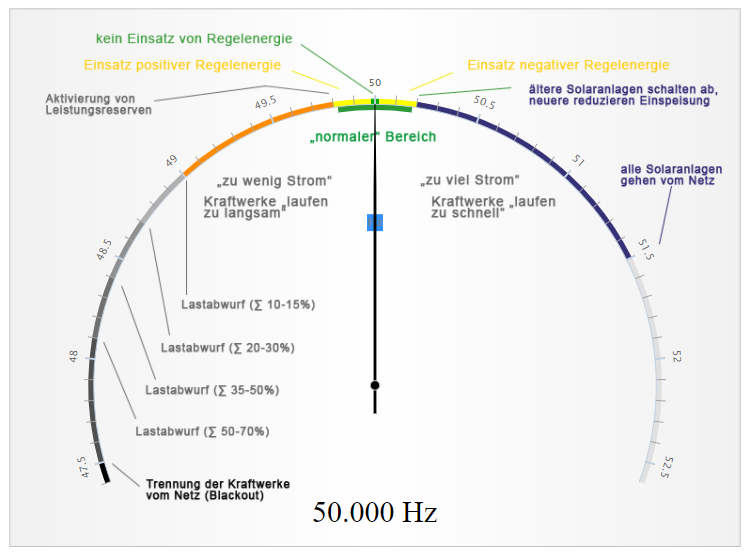
\includegraphics[width=0.9\textwidth]{images/Frequenz.png}
  \end{figure}
%Quelle:http://www.netzfrequenz.info/aktuelle-netzfrequenz-full
\end{frame}
}

\begin{frame}{Regelung der Netzfrequenz}
Notwendigkeit von Regelbarer Leistung um Frequenz konstant zu halten
\begin{itemize}
  \item positive Regelenergie:
  \begin{itemize}
    \item[-] mehr Strom muss in das Netz eingespeist werden
    \item[-] weniger Strom muss verbraucht werden
  \end{itemize}
  \item negative Regelenergie:
  \begin{itemize}
    \item[-] Stromeinspeisung muss schnell reduziert werden
    \item[-] mehr Strom muss verbraucht werden
  \end{itemize}
  \item[\rightarrow] Kraftwerke oder Verbraucher mit einer diesen Eigenschaften eignen sich um Regelenergie bereitzustellen
\end{itemize}
\end{frame}

\begin{frame}
  \begin{itemize}
    \item Primärregelung PRL
    \begin{itemize}
      \item[-] automatische vollständige Aktivierung innerhalb von \SI{30}{\second}
      \item[-] abzudeckender Zeitraum \num{0}<\SI{15}{\minute}
      \item[-] Bereitstellung durch alle ÜNB im ENTSO-E-Gebiet
      \item[-] Frequenzabhängige Lasten Vorteilhaft z. B. ?Asynchronmotor?
      \item[-] ?keine Unterscheidung zwischen positiver und negativer Regelenergie?
    \end{itemize}
    \item Sekundärregelung SRL
    \begin{itemize}
      \item[-] automatische Aktivierung durch betroffenen ÜNB
      \item[-] vollständige Aktivierung innerhalb von \SI{5}{\minute}
      \item[-] Unterscheidung zwischen positiver und negativer Regelenergie
      \item[-] Breitstellung durch z. B. Pumpspeicherkraftwerken, Gasturbinen, Biogasanlagen oder Blockheizkraftwerke
    \end{itemize}
    \end{itemize}

\end{frame}


{
\setbeamertemplate{footline}{}
\begin{frame}
\begin{itemize}
\item Tertiärregelung(Minutenreserve) MRL
\begin{itemize}
  \item[-] Aktivierung innerhalb von \SI{15}{\minute}
  \item[-] abzudeckender Zeitraum mehrere Stunden bei Störungen
  \item[-] Unterscheidung zwischen positiver und negativer Regelenergie
  \item[-] Breitstellung durch Kraftwerke identisch zu SRL oder Verbraucher deren Lasten abgeworfen werden
\end{itemize}
\end{itemize}

  \begin{figure}
  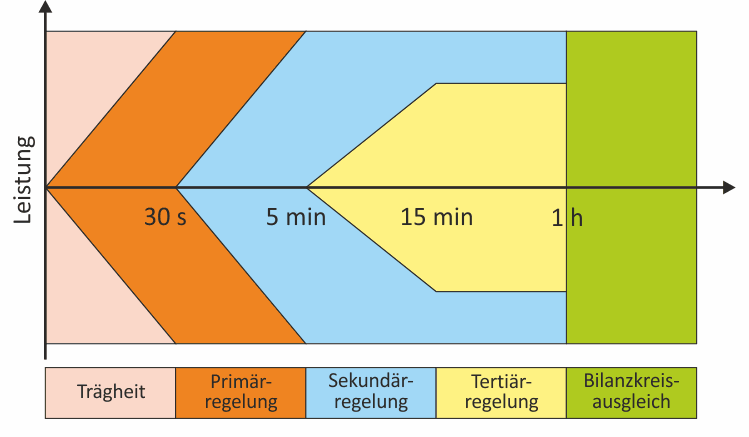
\includegraphics[width=0.7\textwidth]{images/Regelleistung.png}
\end{figure}
%Quelle:https://fenecon.de/page/stromspeicher-energy-pool
\end{frame}
}


\begin{frame}{Paradigmenwechsel}
\begin{itemize}
  \item Stromindustie und auch Verbraucher
  steht vor bsw. befinden sich
  in einem Paradigmenwechsel hervorgerufen durch die Energiewende
\end{itemize}
%
 \begin{tabular}{p{0.5\textwidth}p{0.5\textwidth}}
 \textbf{\textcolor{tugreen}{ Ursprüngliche Situation:}}

 \begin{itemize}
     \item[-] Kraftwerkleistungen werden an Lastprofil angepasst
     \item[-] Lastprofil der Verbraucher bekannt und wenig fluktuierend
         \item[$\rightarrow$] geringe Schwankungen der Netz-Frequenz
         \item[$\rightarrow$] geringer Einsatz von Regelenergie
   \end{itemize}
 &
 \textbf{\textcolor{tugreen}{Neue Situation:}}
    \begin{itemize}
      \item[-] Erneuerbare Energie wird zum größten Teil aus volatilen Quellen wie Wind und Sonne gewonnen
      \item[-] Nur wenige Grundlastfähige EE-Quellen wie Wasserkraft und Biogas
      \item[$\rightarrow$] EE-Kraftwerkleistungen nur noch bedingt oder gar nicht steuerbar
      \item[$\rightarrow$] keine Anpassung an Lastprofil möglich
      \item[$\rightarrow$] Netz-Frequenz fluktuierd stärker
      \item[$\rightarrow$] hoher Einsatz von Regelenergie, um Netzstabilität zu gewährleistern
    \end{itemize}\\
  \end{tabular}
\end{frame}


\begin{frame}{Folgen der Energiewende auf Stromnetz}
  \begin{tabular}{p{0.5\textwidth}p{0.5\textwidth}}
\textbf{\textcolor{tugreen}{Ursprüngliches Stromnetz:}}
\begin{itemize}
  \item Großkraftwerke wie z. B. Kern- oder Braunkohlekraftwerke,
  welche eine Region mit Strom versorgen
  \item "Einbahnstraße im Stromnetz"
\item[$\rightarrow$]  Kraftwerk$\rightarrow$Stromnetz$\rightarrow$Verbraucher
\item[$\rightarrow$]  Höchspannung$\rightarrow$Niederspannung
\end{itemize}
&
\textbf{\textcolor{tugreen}{Neues Stromnetz:}}

\begin{itemize}
  \item Erneuerbare Energiequellen können
  sowohl zentral z.B. Offshore Windparks als auch
  dezentral beim Verbraucher selbst
  produzierte werden
\item[$\rightarrow$]  Kraftwerk$\rightarrow$Stromnetz$\leftrightarrows$Verbraucher
\item[$\rightarrow$]  Höchstspannung$\leftrightarrows$Niederspannung
\end{itemize}
\end{tabular}
\begin{itemize}
  % \textbf{\textcolor{tugreen}{Fazit:}}
\item[Fazit:] Notwendigkeit des Netz-um/aus-bau durch Energiewende
damit eine sichere Versorgen gegeben bleibt.
\item[$\rightarrow$] Netzentwicklungsplan NEP 2017-2030 der Bundesnetzagentur
\end{itemize}

\end{frame}



{
\setbeamertemplate{footline}{}
 \begin{frame}{Netzausbau}
%     \begin{figure}
%     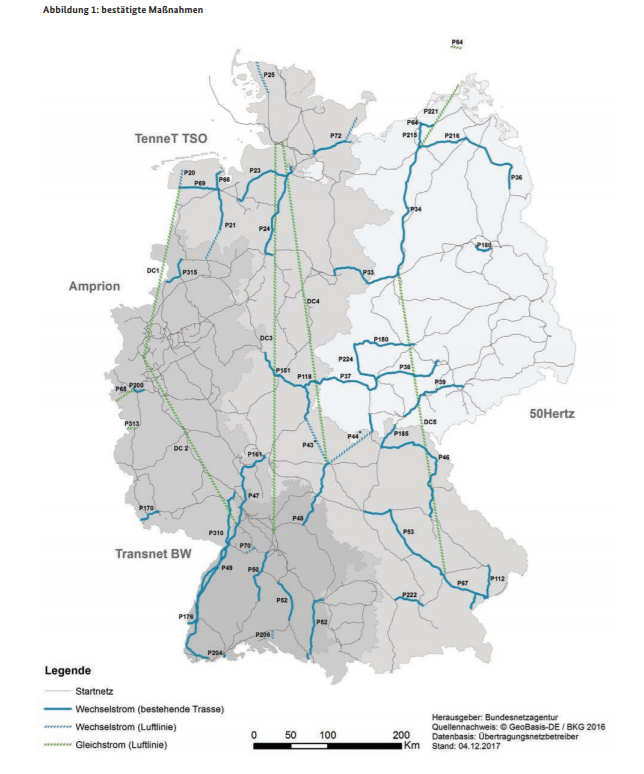
\includegraphics[width=0.55\textwidth]{images/Ausbau.PNG}
%   \end{figure}
\begin{overpic}[width=0.5\textwidth,tics=10]
{images/Ausbau.jpg}
\put(80,10){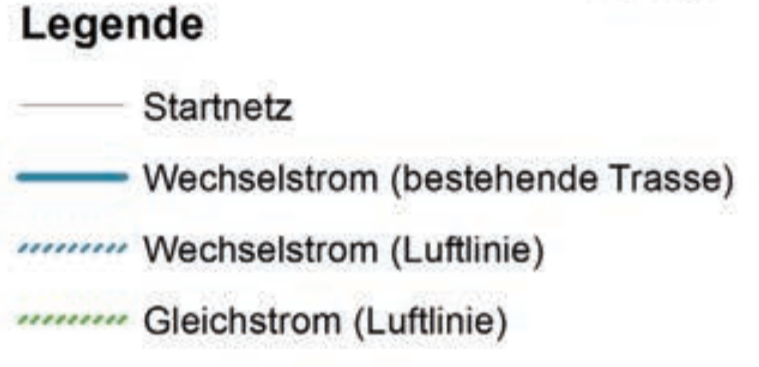
\includegraphics[scale=0.5]{images/Legende_deutschland.PNG}}
\end{overpic}
\end{frame}
}





{
\setbeamertemplate{footline}{}
 \begin{frame}{Netzausbau}
%     \begin{figure}
%     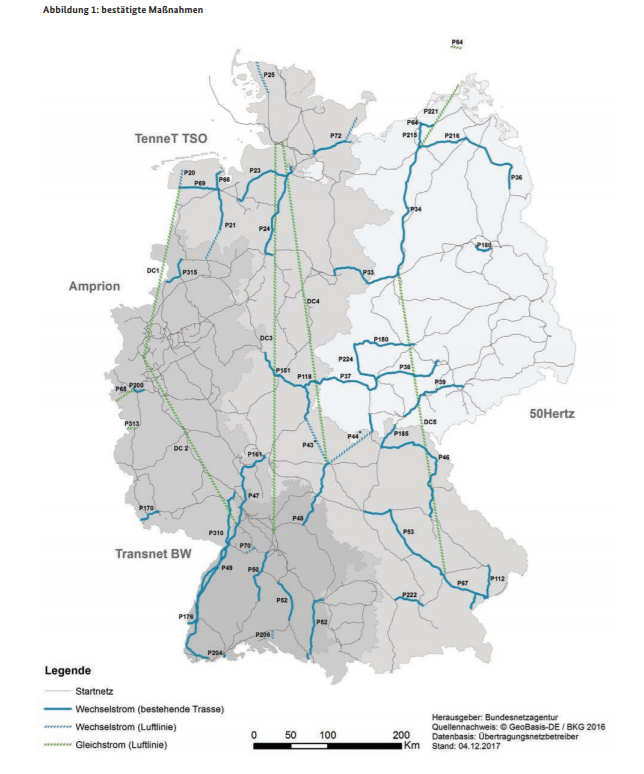
\includegraphics[width=0.55\textwidth]{images/Ausbau.PNG}
%   \end{figure}
\begin{overpic}[width=0.5\textwidth,tics=10]
{images/NAusbau1.jpg}
\put(80,10){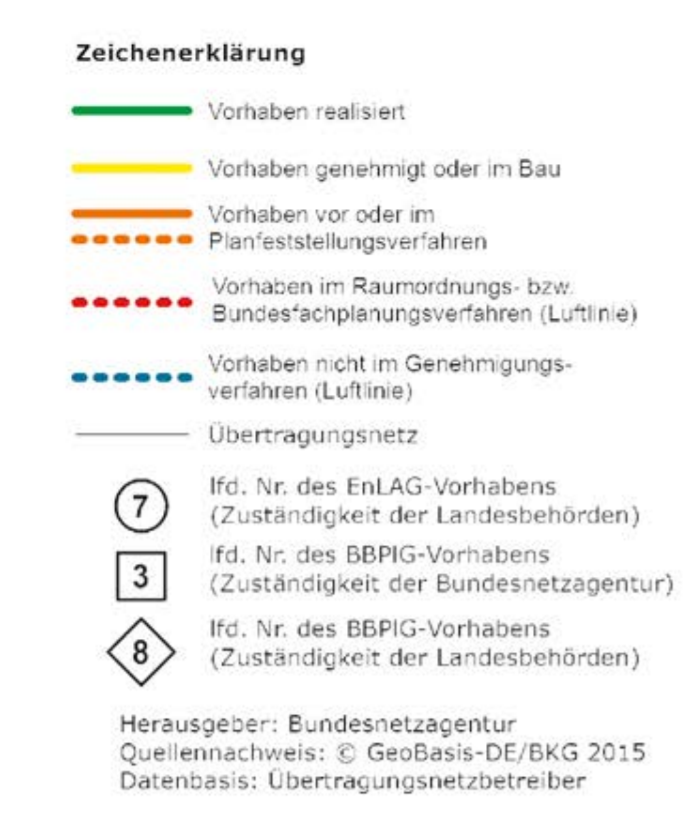
\includegraphics[scale=0.5]{images/NLegende.PNG}}
\end{overpic}
\end{frame}
}

\begin{frame}{Zukunft Smart-Gird}
\begin{itemize}
  \item intelligentes Stromnetz durch durch Energiewende und
   die damit einhergehenden Volatile Stromerzeuger nötig
  \item Smart-Gird bietet Möglichkeit zu
  verfügungstehenden Strom effektiv zu nutzen
  \item Datenaustausch zwischen Netzbetreiber,
       Verbraucher und Erzeuger z. B. Smart-Meters in Haushaltens
  \item[\rightarrow] mehr Kontrolle und Information
   für die Netzbetreiber für besseres Lastmanagement
   \item zusätzlich Anpassung der Nachfrage in Haushalten (Smart-Houses)
 \end{itemize}
\end{frame}

\begin{frame}
\begin{figure}
  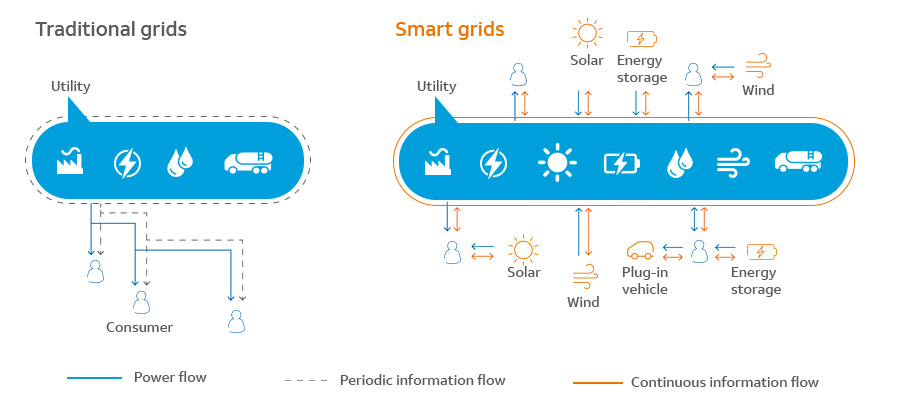
\includegraphics[width=1\textwidth]{images/smart-grid.jpg}
  %https://www.business.att.com/solutions/Service/internet-of-things/smart-cities/iot-smart-grid/
\end{figure}
\end{frame}

\begin{frame}{Blackout}
  \begin{columns}
\begin{column}{0.5\textwidth}
\begin{itemize}
\item totaler Stromausfall mit regionale bis überregionalen Auswirkungen
\item Ursachen:
\item[-]meist Vernachlässigung des $N-1$-Kriterium z.B. Ems-Freileitungskreuzung
\item[-]extreme Wetterbedingungen z.B. Münsterländer Schneechaos
\item[-]sabotierende Angriffe gegen Stromnetz oder Kraftwerke
   z.B. fiktiver Thriller Blackout - Morgen ist es zu spät von Marc Elsberg
\end{itemize}
\end{column}
\begin{column}{0.5\textwidth}
  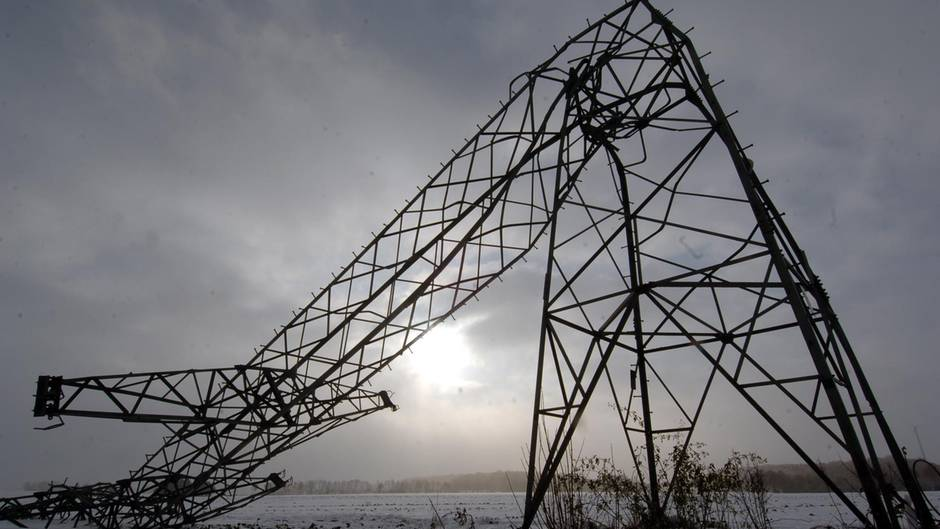
\includegraphics[width=1\textwidth]{images/stromausfall-deutschland-muensterland.jpg}\\
\end{column}
\end{columns}
\end{frame}





\begin{frame}{Strombörse}
\begin{itemize}
  \item existiert seit \num{2000} in Europa
  \item Strombörsen in Europa koordiniert von der EEX Group
  \item Deutschland, Frankreich, Österreich
  und Schweiz handeln an European Energy Exchange (EEX) in Leipzig
 und European Power Exchange (EPEX SPOT) in Paris
 \item Unterscheidung zwischen Spotmarkt, Terminmarkt und Regelenergiemarkt
\item Gehandelte Produkte zusätzlich zu Strom:
    \begin{itemize}
      \item[-]Öl, Gas, Kohle, Metall, Frachtprodukte,
       Emissionsberechtigungen sowie Agrarprodukte
    \end{itemize}
\end{itemize}
\end{frame}


{
\setbeamertemplate{footline}{}
\begin{frame}
  \begin{figure}
  \includegraphics[width=1.1\textwidth]{images/stromprodukte.jpg}
\end{figure}
%Quelle:https://www.next-kraftwerke.de/wissen/strommarkt/spotmarkt-epex-spot
\end{frame}
}

\begin{frame}{Spotmarkt}
  \begin{columns}
  \begin{column}{0.3\textwidth}
  \begin{itemize}
    \item Spotmarkt in Paris an der EPEX SPOT
    \item Handel von kurzfristig lieferbaren Strommengen in bestimmten Blöcken
    \item Im Intraday-Handel (Lieferung am selben Tag)
    \item Im Day-Ahead-Handel (Lieferung am Folgetag)
  \end{itemize}
  \end{column}
  \begin{column}{0.7\textwidth}
  \begin{figure}
  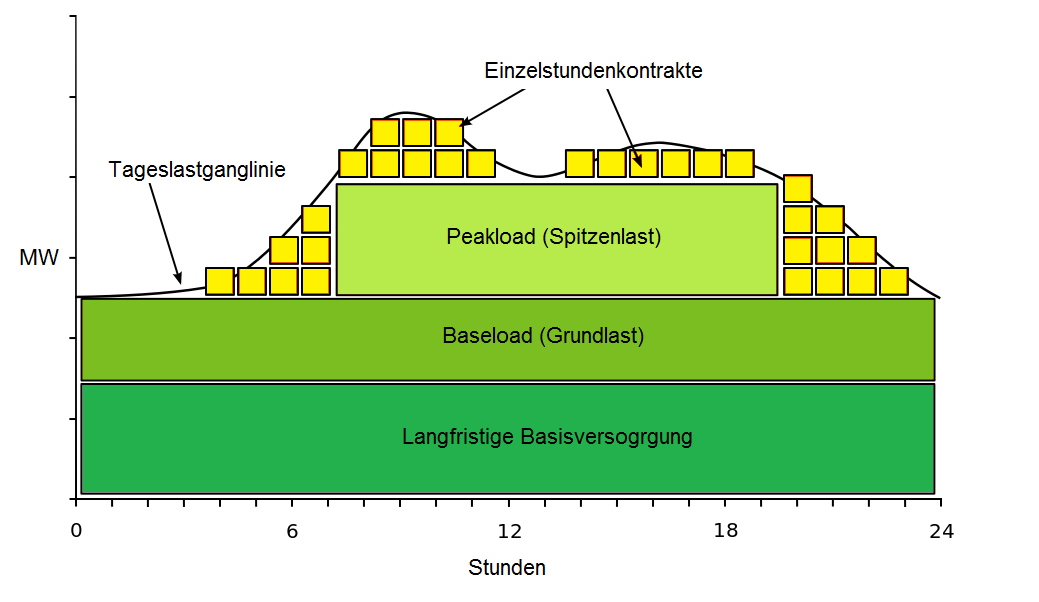
\includegraphics[width=1\textwidth]{images/Stromborse_stromverbrauch_lastprofil.png}
  \end{figure}
\end{column}
\end{columns}
\end{frame}


\begin{frame}{Merit-Order}
\begin{itemize}
  \item Beschreibungsmodell der Preisbildung auf dem Strommarkt
  \item orientiert sich an den Grenzkosten der Kraftwerke
  (Grenzkosten entspricht kosten für die letzte produzierte Megawattstunde)
\item Kraftwerke mit niedrigen Grenzkosten werden bei der
 Einspeisung bevorzugt, bis Nachfrage gedeckt ist
\item Börsenpreis ergibt sich aus Schnittstelle von Angebot und Nachfrage
\begin{itemize}
  \item[$\rightarrow$] Grenzkosten des Kraftwerkes, welches zuletzt den
  Zuschlag zur Einspeisung erhält, definiert Börsenpreis für alle eingespeisten Kraftwerke("uniform pricing")
\end{itemize}
\end{itemize}
\begin{tabular}{p{0.4\textwidth}p{0.6\textwidth}}
&
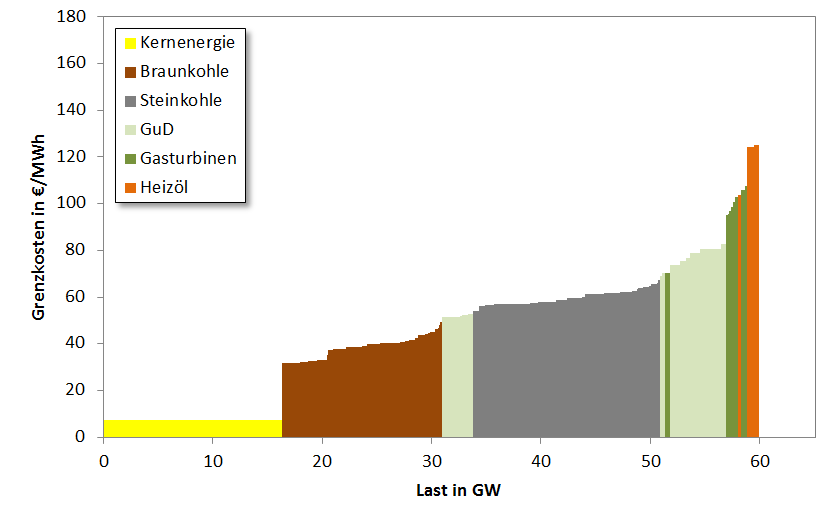
\includegraphics[width=0.5\textwidth]{images/Merit_Order_2008.PNG}
\\
\end{tabular}
\end{frame}

\begin{frame}
  \begin{figure}
  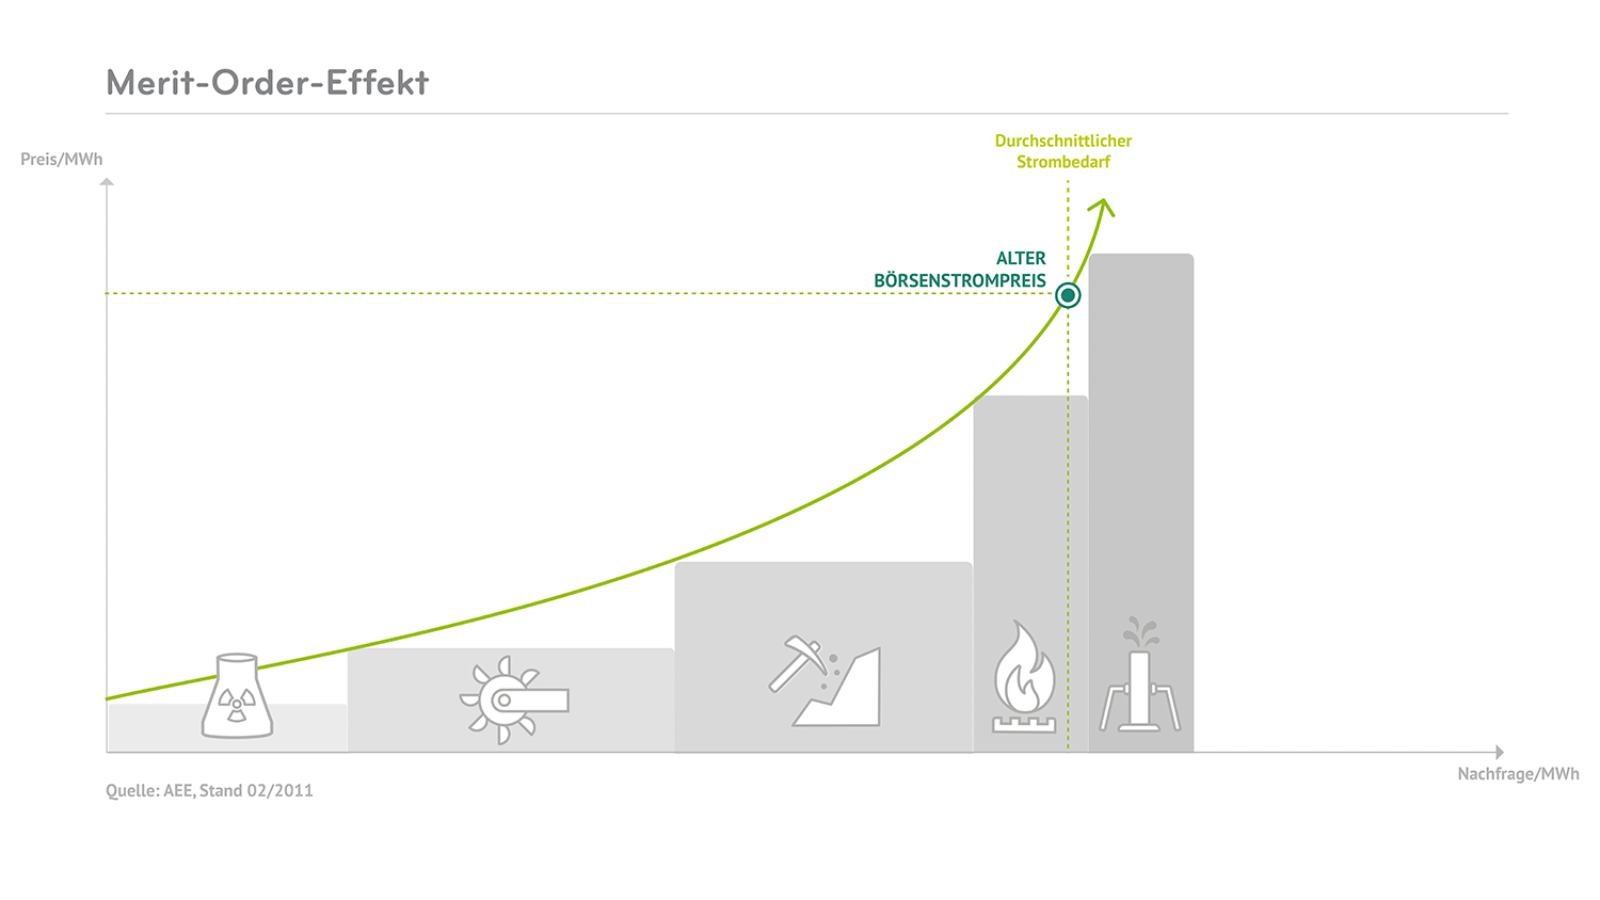
\includegraphics[width=1\textwidth]{images/Meritorder.png}
\end{figure}
%Quelle:https://www.next-kraftwerke.be
\end{frame}


\begin{frame}
  \begin{figure}
  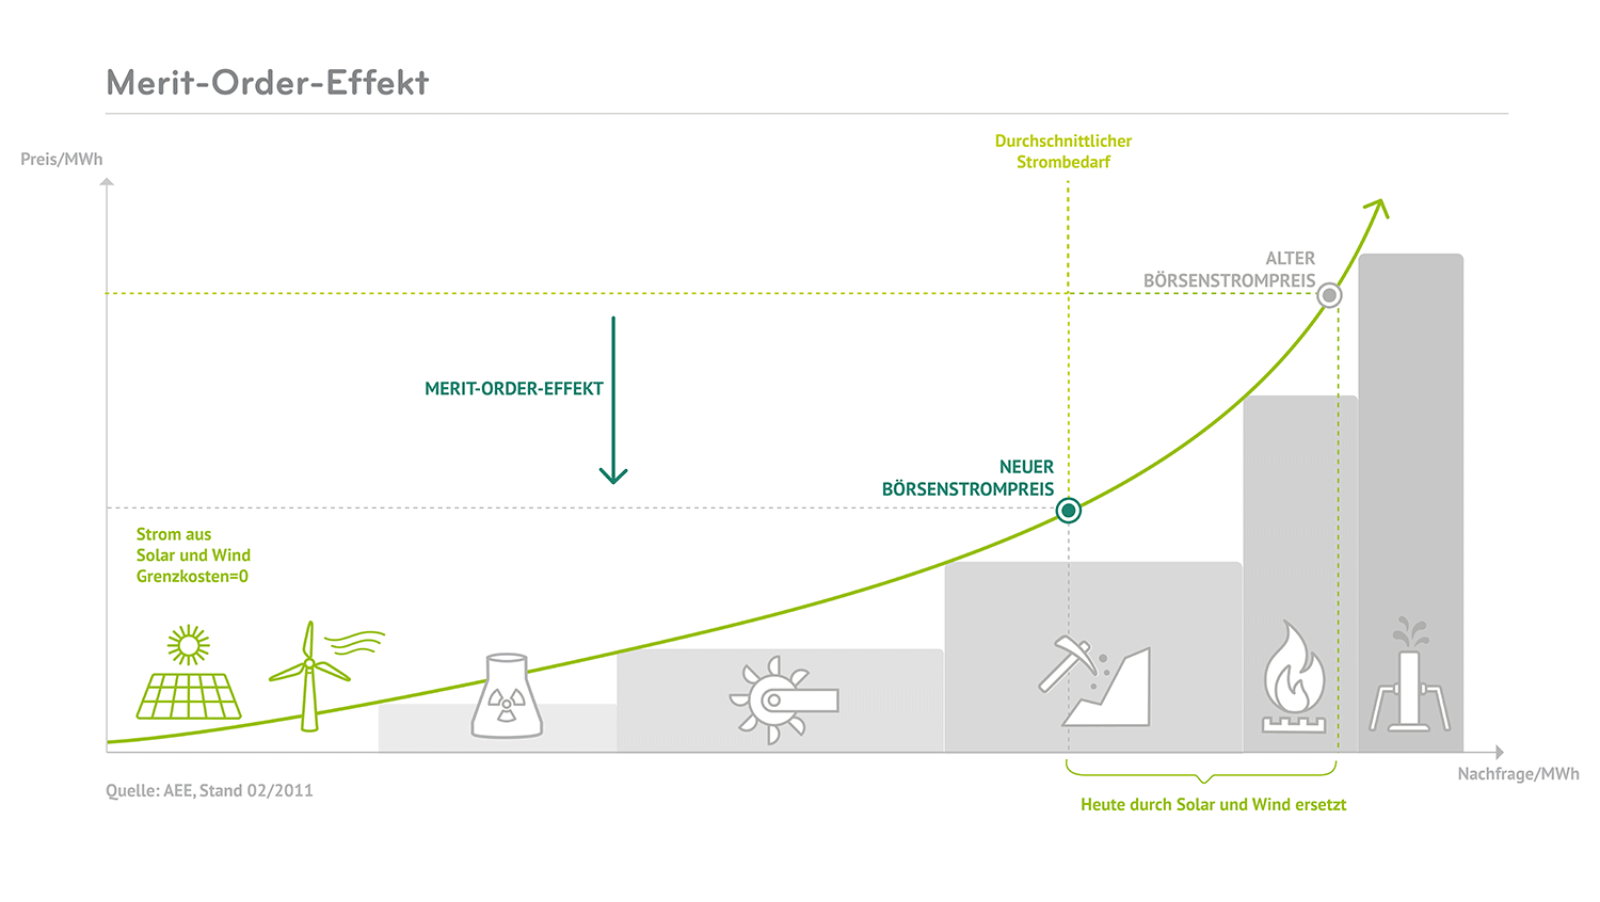
\includegraphics[width=1\textwidth]{images/Merit.png}
\end{figure}
%Quelle:https://www.next-kraftwerke.be
\end{frame}


\begin{frame}
  \begin{figure}
  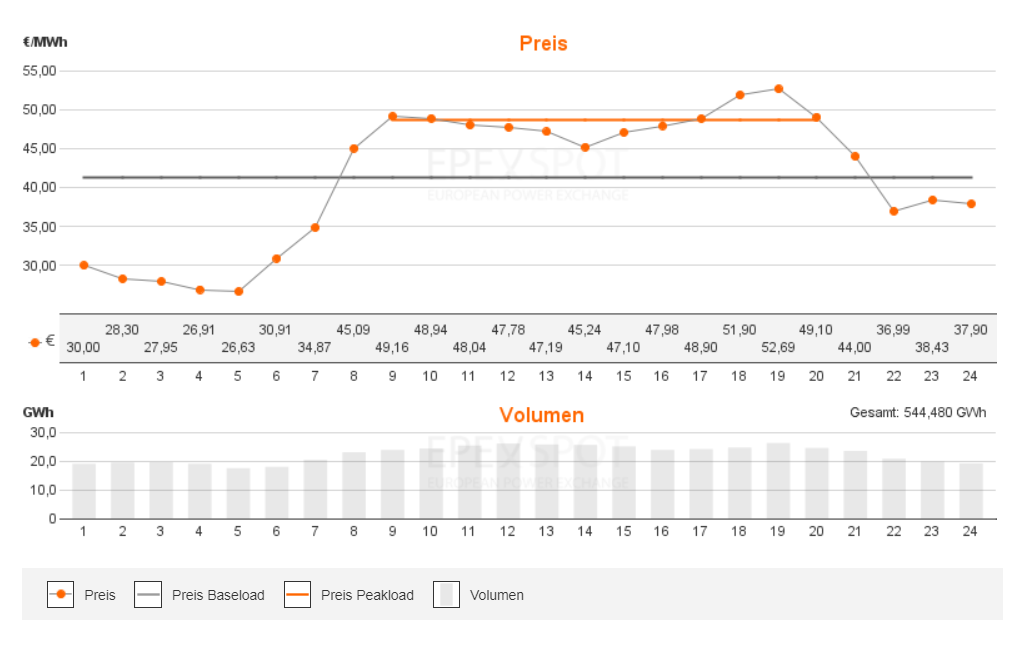
\includegraphics[width=0.9\textwidth]{images/10_1_2018_spot.PNG}
\end{figure}
\end{frame}

\begin{frame}{Terminmarkt}
\begin{itemize}
  \item Terminmarkt in Leipzig an der EEX
  \item Handel von Strommengen, die zu einem festen Termin zu Verfügung gestellt werden (Strom-Futures)
  \item bis zu 6 Jahre Strom im voraus kaufen
  \item Jahr-, Quartal-, Monat-, Woche-,  Wochenende- und Tag-Kontrakte
  \item Preis richtig sich an Börsenindex der Strombörse z. B. Phelix (Physical Electricity Index)
\end{itemize}
\end{frame}

\begin{frame}
  \begin{figure}
  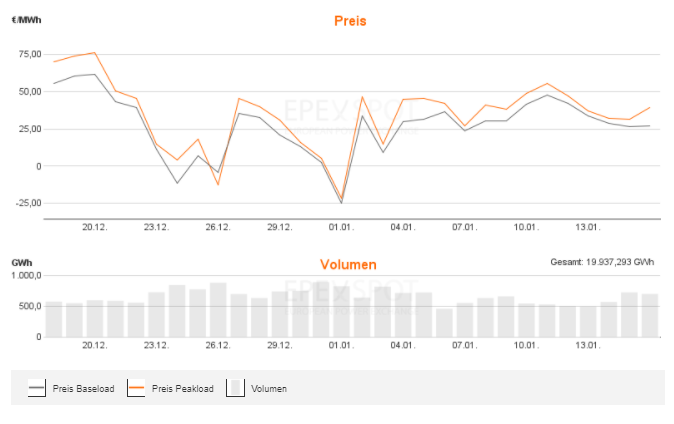
\includegraphics[width=0.9\textwidth]{images/Phelix_1monat.PNG}
\end{figure}
\end{frame}


\begin{frame}{Regelenergiemarkt}
\begin{itemize}
  \item Bedarf an Regelenergien von PRL, SRL und MRL werden durch Ausschreibung
der ÜNB gedeckt
\item PRL und SRL werden jede Woche neu ausgeschrieben
\item MRL werden Täglich neu ausgeschrieben und nach Merit-Order-Liste bei Bedarf abgerufen
\item Preis abhängig von Verträgen zwischen Anbieter und ÜNB
\end{itemize}
\end{frame}


\begin{frame}
  \begin{figure}
  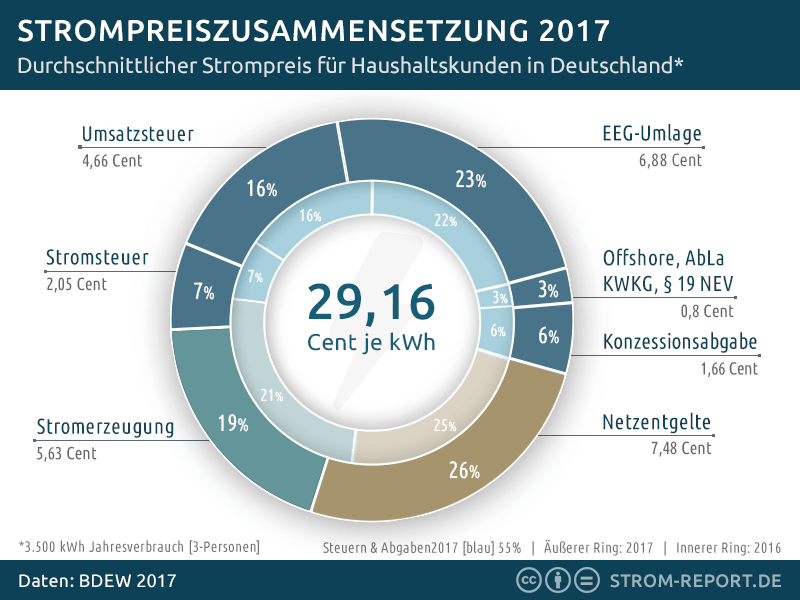
\includegraphics[width=0.9\textwidth]{images/strompreis-zusammensetzung.png}
  \end{figure}
\end{frame}



\begin{frame}{Erneuerbare-Energien-Gesetz EEG}
   \begin{itemize}
     \item das EEG wurde im Jahr 2000 eingeführt und mehrmals überarbeitet aktuell EEG 2017
   \end{itemize}
\pause
    \begin{block}{Ziel:}
      Förderung von Erneuerbaren Energiequellen, damit Umstieg von Konventionellen zur Erneuerbaren Energiequellen gelingt
    \end{block}
  %\item Regelt die Einspeisung des EE-Stromes
\pause
    \begin{block}{Maßnahmen des EEG zu Förderung von EE-Strom:}
     \begin{itemize}
       \item[$\rightarrow$] Verpflichtung an die Netzbetreiber EE-Anlagen an das Stromnetz anzuschießen und EE-Strom vorrangig einzuspeisen
       \item[$\rightarrow$] garantierte Einspeisevergütung des EE-Stromes an die Anlagenbetreiber durch den Netzbetreiber für 20 Jahre
   \end{itemize}
   \end{block}
\end{frame}

\begin{frame}{Auswirkungen des EEG}
  \begin{itemize}
    \item Abnahmepflicht fördert Merit-Order-Effekt
    \item Netzbetreiber bieten abgenommenen EE-Strom an der Börse an
\begin{itemize}
  \item[$\rightarrow$] Gewinn an der Strombörse deckt jedoch nicht die vollen Vergütungskosten der Netzbetreiber
\end{itemize}
\end{itemize}
\begin{block}{EEG-Umlage}
\begin{itemize}
  \item $\text{EEG-Umlage}=\text{Einspeisevergütung}-\text{Börsengewinn}$
\item die EEG-Umlage erhält der Netzbetreiber von allen Stromverbrauchern
\item Strompreis enthält die EEG-Umlage
\end{itemize}
\end{block}
\end{frame}

{
\setbeamertemplate{footline}{}
\begin{frame}
  \begin{figure}
  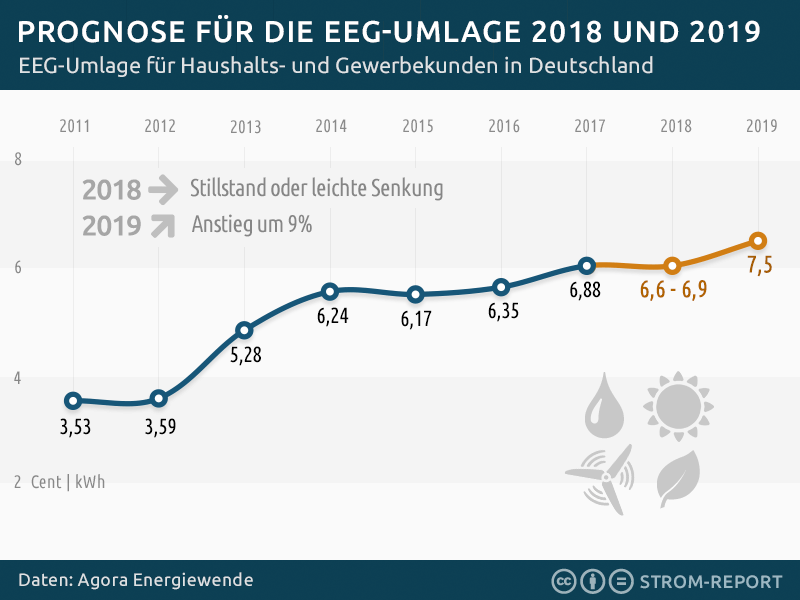
\includegraphics[width=0.9\textwidth]{images/eeg-umlage-2018-2019.png}
  \end{figure}
%Quelle:https://1-stromvergleich.com/strom-report/eeg-umlage/#eeg-umlage-2018
\end{frame}
}




{
\setbeamertemplate{footline}{}
\begin{frame}
  \begin{figure}
  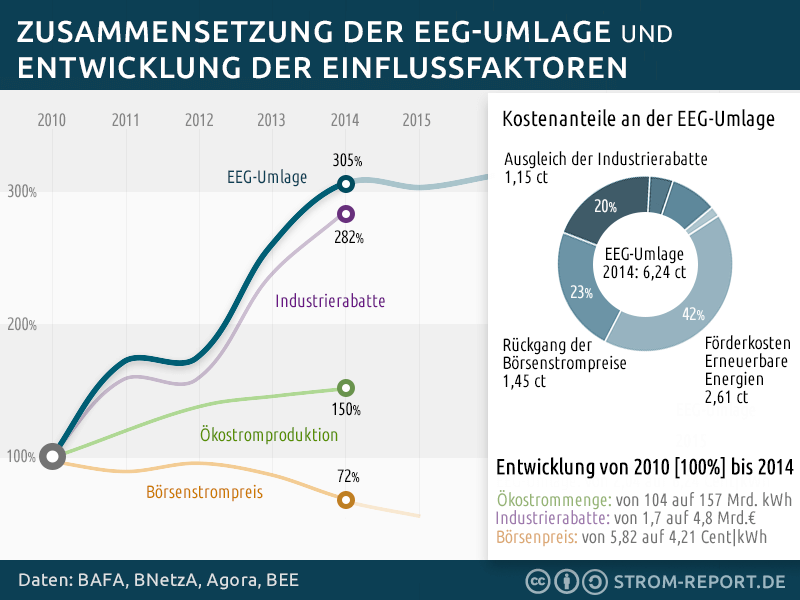
\includegraphics[width=0.9\textwidth]{images/eeg-umlage.png}
  \end{figure}
%Quelle:https://1-stromvergleich.com/strom-report/eeg-umlage/#eeg-umlage-boersenpreis-industrierabatt
\end{frame}
}


\begin{frame}{Entwicklung}

\end{frame}



\begin{frame}{Zusammenfassung}
\begin{tabular}{p{0.4\textwidth}p{0.6\textwidth}}
   Stormnetz  &         Strombörse\\
\begin{itemize}
  \item Dreiphasiger Wechselstrom in Verbundnetzen
  \item 4 Spannungsebenen
  \item keine Energiespeicherung im Netz selber möglich
  \item Netzfrequenz durch Regelleistung geregelt
  \item Paradigmenwechsel in der Stromindustrie durch Energiewende
  \item Netzausbau und neue Konzepte nötig um Energiewende zu bewergstellen
\end{itemize}

&
\begin{itemize}
  \item Unterscheidung zwischen Spot-, Termin- und Regelenergiemarkt
  \item Preisbildung an dem Spotmarkt durch die Merit-Order
  \item Merit-Order-Effekt durch EE
  \item EEG als Beschleuniger der Energiewende und seine Folgen
\end{itemize}

\end{tabular}
\end{frame}


\begin{frame}{Backup}

\end{frame}
\begin{frame}{Quellen}

\end{frame}
%
% {
% \setbeamertemplate{footline}{}
% \begin{frame}
%   \begin{figure}
%   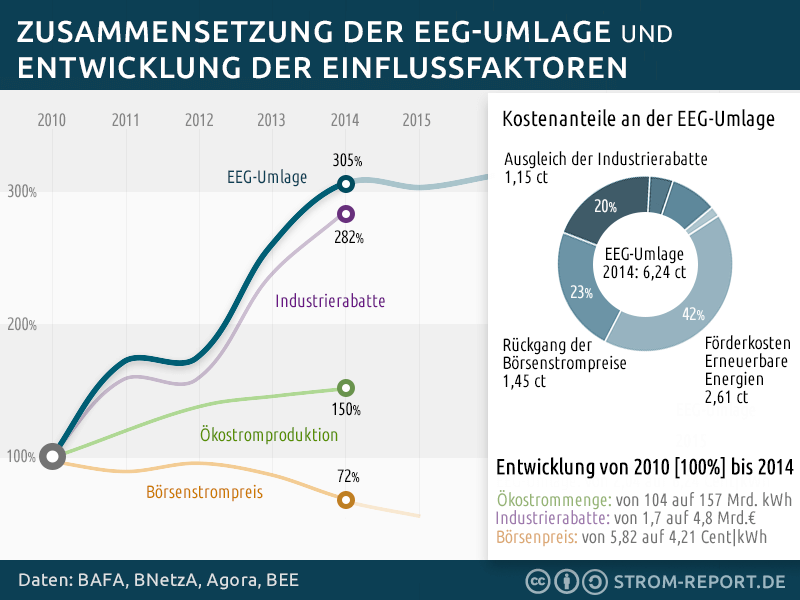
\includegraphics[width=0.9\textwidth]{images/eeg-umlage.png}
%   \end{figure}
% %Quelle:https://1-stromvergleich.com/strom-report/eeg-umlage/#eeg-umlage-boersenpreis-industrierabatt
% \end{frame}
% }




\end{document}
